\documentclass{beamer}

\usepackage{svg}

\usetheme{Boadilla}
\usecolortheme{dolphin}
\usepackage[style=ieee]{biblatex}
\setbeamertemplate{navigation symbols}{}
\setbeamertemplate{sections/subsections in toc}[sections numbered]

\setbeameroption{hide notes}
\addbibresource{ref.bib} %Imports bibliography file
% \setbeameroption{show only notes}
% \setbeameroption{show notes on second screen=right}

\title[ETM-Guided MBTA]
{An ETM-Guided Measurement-Based Timing Analysis in
Embedded Systems}
\author[Hossein Afkar]{Hossein Afkar \\ \footnotesize Supervised by: Dr. Kargahi}
\institute{University Of Tehran}
\titlegraphic{
\includegraphics[width=1.85cm]{ut.png}
\includegraphics[width=2cm]{drts.png}}
\date{\today}

\begin{document}

\setbeamertemplate{footnote}{%
  \parindent 1em\noindent%
  \raggedright
  \insertfootnotetext\par%
}

\frame{\titlepage}

\begin{frame}
    \frametitle{Outline}
    \tableofcontents[hideallsubsections]
\end{frame}

\section{Introduction}
\begin{frame}
    \frametitle{Introduction}
    \begin{columns}[c]
        \column{3.5in}
        \begin{itemize}
            \item Cyber-physical systems:
                \begin{itemize}
                    \item Interplay between digital and physical realms.
                        \nocite{lee2008cyber}
                    \item High economic and social potential.
                \end{itemize}
            \item Design Implications:
                \begin{itemize}
                    \item Reliability.
                    \item Predictability.
                \end{itemize}
        \end{itemize}
        \column{1.5in}
        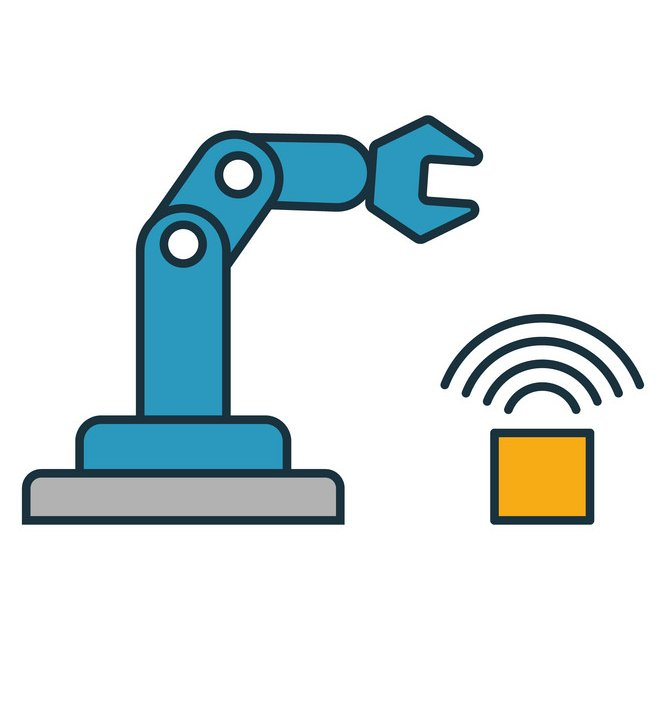
\includegraphics[width=1in]{cps.jpg}
    \end{columns}
\end{frame}
\section{Defining Research}
\begin{frame}
    \frametitle{Defining Research}
    \begin{itemize}
        \item Modeling requires accurate and tight estimates
            of Worst-Case Execution Time (WCET).
            \nocite{gustafsson2010malardalen}
            \nocite{schlatow2018data}
        \item Various ways have been used in the calculation of WCET:
            \begin{itemize}
                \item Static Analysis
                    \begin{itemize}
                        \item Increased difficulty in complex architectures.
                        \item Pessimistic.
                    \end{itemize}
                \item Measurement-based.
                \item Hybrid.
            \end{itemize}
        \item Challenges:
            \begin{itemize}
                \item Test vector generation.
                \item Context-dependece.
                \item Overhead.
            \end{itemize}
        \item Automotive control systems are constrained by Sensor-to-Actuator
            delays.
            \begin{itemize}
                \item Sensor data age becomes apparent.
            \end{itemize}
    \end{itemize}
    \nocite{shah2014measurement}
    \nocite{bunte2011let}
\end{frame}
\section{Method}
\begin{frame}
    \frametitle{Method}
    \begin{itemize}
        \item Main focus is on measurement-based timing analysis:
            \begin{itemize}
                \item Using Embedded Trace Macrocell (ETM) we can gather
                    real-time and cycle-accurate traces from the processor.
                \item Use MEM-AP from ARM Debug Interface to supply test
                    vectors and to automate the workflow.
            \end{itemize}
        \item Our secondary focus is the sensor data age measurement:
            \begin{itemize}
                \item Construct a Data Dependency Graph and use ETM data-trace to
                    add data dependencies that are determined during runtime.
                \item Use Data Dependency Graph and ETM to measure sensor data
                    age.
            \end{itemize}
            \nocite{macrocell2007etmv1}
    \end{itemize}
\end{frame}
\section{Literature Review}
\begin{frame}
    \frametitle{Literature Review}
    How our work differs according to the literature review:
    \begin{itemize}
        \item A new tool for measurement-based timing analysis
            \begin{itemize}
                \item No added instrumentation points.
                \item Data age measurement.
                \item Enforcing predictable hardware and software state.
            \end{itemize}
        \item Sensor data age:
            \begin{itemize}
                \item Add dynamic dependencies to DDG using ETM.
                \item Use an annotated DDG to measure the sensor data age
                    using ETM.
            \end{itemize}
        \item Output from this research can be used in the cause-effect chain
            analysis and schedulability analysis of real-time systems.
    \end{itemize}
\end{frame}
\section{References}
\begin{frame}[allowframebreaks]
    \frametitle{References}
    \printbibliography
\end{frame}
\begin{frame}
  \centering \Large
  \emph{Thank You For Your Attention}
\end{frame}

\end{document}
